\section{Properties of Crystals}

\subsection{Introduction}

There are seven crystal classes, although this work is only concerned with cubic and orthorhombic crystals.  

\begin{table}[h]
\caption{Seven Crystal Classes}
\begin{center}
\begin{tabular}{c c c}
Class & Lengths & Angles \\
\hline\hline
Cubic & $a = b = c$ & $ \alpha = \beta = \gamma = 90^{\circ}$ \\
Hexagonal & $a = b, c $ & $ \alpha = \beta, \gamma = 120^{\circ}$ \\
Rhombohedral & $a = b = c $ & $ \alpha = \beta = \gamma \neq 90^{\circ}$ \\
Tetragonal & $a = b, c $ & $ \alpha = \beta = \gamma = 90^{\circ}$ \\
Orthorhombic & $a, b, c $ & $ \alpha = \beta = \gamma = 90^{\circ}$ \\
Monoclinic & $a, b, c $ & $ \alpha = \beta = 90^{\circ}, \gamma \neq 90^{\circ} $ \\
Triclinic & $a, b, c $ & $ \alpha, \beta, \gamma, $ \\
\end{tabular}
\end{center}
\end{table}




The force matching method uses DFT calculated forces as well as other properties, calculated either by DFT or measured by experiment, in order to fit potential functions.  These additional constraints include:

\begin{itemize}
\item Lattice Parameter $a_0$
\item Cohesive Energy $E_{coh}$
\item Bulk Modulus $B_{0}$
\item Equation of State $(E_{0}, V_{0}, B_0, {B^{p}_0})$
\item Stress Tensor
\item Elastic Constants
\item Shear Modulus, Young's Modulus, Poisson Ratio
\item Melting Temperature
\item Surface Energy
\end{itemize}


\subsection{Bulk Modulus}

The Bulk Modulus of a material is defined as the bulk stress of a sample divided by the bulk strain on that sample.  It is also the inverse of the compressibility of that material, which means that materials with a higher bulk modulus are less compressible than those with a lower value.

\eqBulkModulusA

\eqBulkModulusB



\begin{table}[h]
\caption{Useful Conversion Factors}
\begin{center}
\begin{tabular}{c c}
Material & Bulk Modulus/GPa \\
\hline\hline
Aluminium & 70 \\
Iron (BCC) & 110 \\
Stainless Steel 18-8 & 163 \\
\end{tabular}
\end{center}
\end{table}



\subsection{Equation of State}

The equation of state of a material relates either the pressure on that material as a function of the volume, or the energy of a sample of a material to the volume.  This not only allows one to predict the energy or pressure at a certain volume, but also the minimum energy, relaxed volume and the bulk modulus.



\subsection{Murnaghan Equation of State}

Hooke's law implies a linear relationship between stress and strain.  In practice, where a pressure is applied to a material, the application of Hooke's law is limited \cite{murnaghaneq}.  Muraghan derived a new equation to improve upon formulae developed in the 1930's, using compression data from high pressure experiments.

\begin{equation}
\begin{split}
P(V) = \frac{B_0}{{B'}_0}\left(\left(\frac{V_0}{V}\right)^{{B'}_0}-1\right)
\end{split}
\label{eq:eqMurnachanEquationofStatePressure}
\end{equation}

As pressure is the negative derivative of the internal energy of the system with respect to change in volume, $p = -(\partial E/dV)$, and the equation can be integrated and written in terms of the energy, volume, bulk modulus and its derivative\cite{crystaleos}.

\begin{equation}
\begin{split}
E(V) = E_0 + \frac{B_0 V}{{B'}_0} \left[\left(\frac{V_0}{V}\right)^{{B'}_0} \frac{1}{{B'}_0 - 1} + 1 \right] - \frac{B_0 V_0}{{B'}_0-1}
\end{split}
\label{eq:eqMurnachanEquationofStateEnergy}
\end{equation}

\subsection{Birch-Murnaghan Equation of State}

Several years after Murnaghan's equation, Birch developed further upon the experimental data provided by Bridgman.  For cubic symmetry, the description of free energy now includes third order terms in the strain components\cite{birchmurnaghaneq}.

\begin{equation}
\begin{split}
P(V) = \frac{3 B_0}{2} \left[\left(\frac{V_0}{V}\right)^{\frac{7}{3}}-\left(\frac{V_0}{V}\right)^{\frac{5}{3}}\right] \left[1 + \frac{3}{4}({B'}_0-4)\left(\left(\frac{V_0}{V}\right)^{\frac{2}{3}}-1\right)\right]
\end{split}
\label{eq:eqMurnachan Equation of State}
\end{equation}

The energy-volume relationship may again be constructed\cite{crystaleos}.

\begin{equation}
\begin{split}
E(V) = E_0 + \frac{9 V_0 B_0}{16} \left[ \left[ \left(\frac{V_0}{V} \right)^{\frac{2}{3}}-1\right]^{3} {B'}_0 + \left[ \left(\frac{V_0}{V} \right)^{\frac{2}{3}}-1\right]^{2} \left[6 - 4 \left(\frac{V_0}{V} \right)^{\frac{2}{3}}\right] \right]
\end{split}
\label{eq:eqMurnachanEquationofStateVolume}
\end{equation}



\subsection{Fitting Method}

The first step is to fit a second order polynomial to the energy-volume data.  This may be achieved using least-squares fitting with a vandermode matrix.  The coefficients from this polynomial may then be used to calculate reasonable value for $E_0$, $V_0$ and $B_0$; sane starting values of ${B'}_0$ are between 1 and 10, and the code takes a starting value of 2\cite{gilgamesheos}.

\begin{equation}
\begin{split}
E(V) = c_0 + c_1 V + c_2 V^2 \\
V_0 = -\frac{c_1}{2c_2} \\
E_0 = c_2 * {V_0}^2 + c_1 V_0 + c_0  \\
B_0 = 2 c_2 V_0 \\
{B'}_0 = 2
\end{split}
\label{eq:eqMurnachanEquationofStateVolume}
\end{equation}

Newton Gauss is then used to minimise $E_0$, $V_0$ and $B_0$ while ${B'}_0 \in {1.0,1.5,2.0,2.5,3.0,3.5,4.0,4.5,5.0,5.5,6.0}$

\begin{equation}
\begin{split}
\left[J^T J\right] P = J^T R
\end{split}
\label{eq:eqMurnachanEquationofStateVolume}
\end{equation}

The parameters with the lowest residual square sum are returned.




\subsection{Strain}

Strain definition.  

\subsection{Stress}

Stress definition .  Stress is measured in Pa, although in this work it may also be measured in either $Ry/Bohr^3$ or $eV/Ang^3$.


\subsection{Voigt Notation}

Where a tensor is symmetric, Voigt notation is used to simplify how the tensor is written.

\voigtexample



\subsection{Elastic Constants}

The Generalized Hooke's law relates the second order stress and strain tensors using a fourth order stiffness tensor.


\eqStiffnessTensor

\eqStrainTensorVoight

elastic constants tensor.  


\subsection{Calculating Elastic Constants for a Cubic Crystal}


Cubic crystals are the most simple class with primitive unit cells having three orthonormal basis vectors.  Four of the most common variants of the cubic crystal are the simple cubic, body centered cubic, face centered cubic and zincblende.

Due to symmetry, a cubic crystal has only three elastic constants.

Applying strains to a cubic crystal \cite{pressuredepmehl} coupled with the calculation of the Bulk Modulus, as already discussed, allows the three independent elastic constants to be calculated.


\eqMehlStrainA

\eqMehlStrainB



\subsection{Calculating Elastic Constants for Orthorhombic Crystal}


The DFT work here includes Palladium and Iron.  The natural arrangement of Pd atoms in a pure sample are FCC within a cubic crystal.  Pure iron at room temperature is BCC, but this work is interested in austenetic stainless steel where the structure of atoms in the alloy are FCC.  When modelling FCC iron using DFT with a non-polarized calculation, the crystal favours a cubic crystal with the atoms fixed in the FCC positions.  When a spin-polarized calculation is computed, with magnetization along the x-axis, the crystal becomes tetragonal (once again, the atoms are fixed in FCC positions).


\begin{center}
\begin{tikzpicture}[scale=0.5]
\printtikzcrystalbcccubic{}
\end{tikzpicture} 
\begin{tikzpicture}[scale=0.5]
\printtikzcrystalbcccubic{}
\end{tikzpicture} 
\end{center}

\eqCubicEC


\eqOrthoRhombicEC


Once the optimised parameters have been determined for the orthorhombic crystal, nine strains are applied to the crystal \cite{DftTiSiRavindran} in order to calculate the nine independent elastic constants.


\eqInternalEnergy


The first three strains applied to the orthorhombic crystal 

\eqDistortionA
\eqDistortionEnergyA

\eqDistortionB
\eqDistortionEnergyB

\eqDistortionC
\eqDistortionEnergyC


Volume conserving monoclinic distortions are then applied to the crystal to calculate the $C_11$, $C_22$ and $C_33$ elastic constants.


\eqDistortionD
\eqDistortionEnergyD

\eqDistortionE
\eqDistortionEnergyE

\eqDistortionF
\eqDistortionEnergyF



\eqDistortionG
\eqDistortionEnergyG

\eqDistortionH
\eqDistortionEnergyH

\eqDistortionI
\eqDistortionEnergyI


\subsection{Elastic Constants: Bulk Modulus, Young's Modulus, Shear Modulus and Poisson Ratio}

The bulk modulus, as noted earlier, is a measure of the effect of strain on stress.  While it may be calculated by taking the second derivative of energu with respect to volume, or by fitting an equation of state, it may also be calculated using the elastic constants of a material or the compliance constants.

The Young's modulus is a measure of the stiffness of a material, and the shear modulus (also know as the modulus of rigidity) 

\begin{equation}
\begin{split}
B_{V} = \frac{1}{9} \left( C_{11} + C_{22} + C_{33} + 2(C_{12} + C_{13} + C_{23}) \right)
\end{split}
\label{eq:eqLennardJones}
\end{equation}

\begin{equation}
\begin{split}
B_{R} = \left( S_{11} + S_{22} + S_{33} + 2(S_{12} + S_{13} + S_{23}) \right)^{-1}
\end{split}
\label{eq:eqLennardJones}
\end{equation}

Calculation by this method is particularly useful for this work, where the FCC iron crystal is orthorhombic, and not cubic.







\subsection{Correlation of Melting Temperature in Metals with Elastic Constants}

There is a correlation between the melting temperature of metals and their elastic constants \cite{ElasticMeltingTemp}.  

\begin{equation}
\begin{split}
T \approx 598.0 + 6.66 \times (C_{11} + C_{22} + C_{33}) - 0.003 * (C_{11} + C_{22} + C_{33})
\text{Where the temperature is in K, and the elastic constants are in GPA}
\end{split}
\label{eq:eqLennardJones}
\end{equation}

\begin{figure}[htbp]
  \begin{center}
    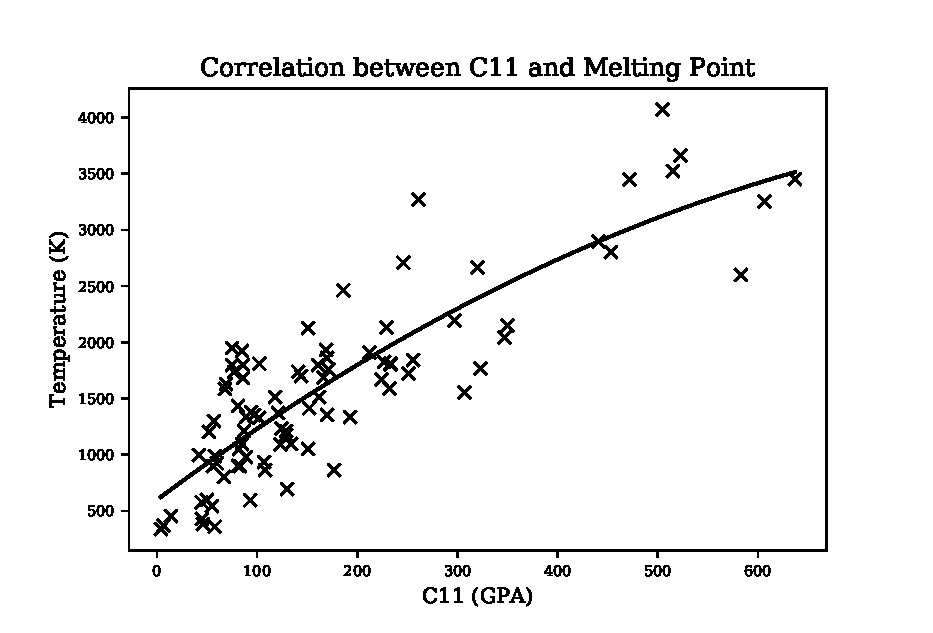
\includegraphics{chapters/background_potential_fitting/plots/c11_temperature}%
    \caption{Graph caption}
    \label{graph:graph1}
  \end{center}
\end{figure}

